%% Журнал ``Квант'', 1970 #3
%% Закон инерции, гелиоцентрическая система и развитие науки
\documentclass[twocolumn,10pt]{article}
\usepackage{pscyr}
\usepackage[cp1251]{inputenc}
\usepackage[T2A]{fontenc}
\usepackage[english,russian]{babel}
\usepackage{ulem}
\usepackage{graphicx}
\graphicspath{{img/}}
\normalem
\begin{document}
\begin{titlepage}
 \begin{center}
  \scalebox{0.7}{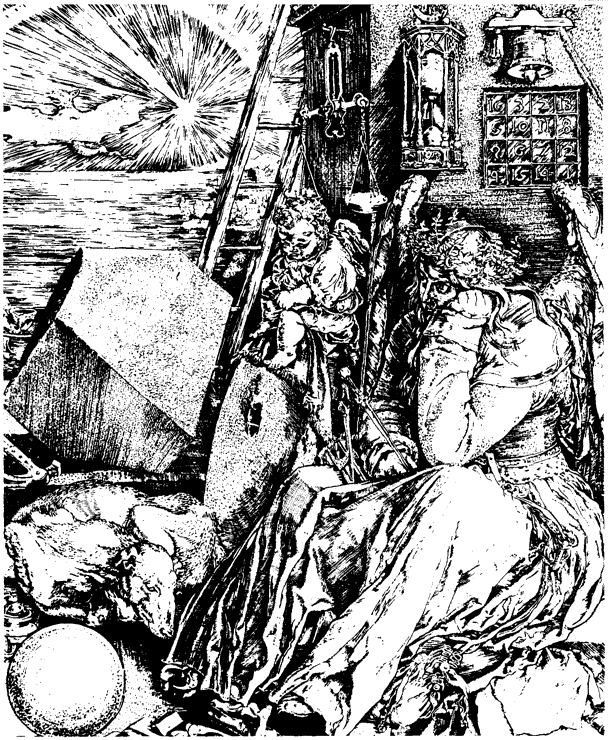
\includegraphics[width=\textwidth]{title.jpg}}

  \textsc{\LARGE{Закон инерции, гелиоцентрическая система и развитие науки}}

  \textsc{\large{М.~Я.~Азбель}}
  \vfill{\large Март~1970}

 \end{center}
\end{titlepage}
\author{М.~Я.~Азбель}
\date{Март~1970}
Характер развития науки драматичен. Но на большом историческом расстоянии даже крупные мазки на полотне науки сливаются, противоречия становятся незаметными, и развитие науки кажется последовательным, строго логичным и все время направленным в одну сторону. На малом расстоянии наука по-настоящему понятна только профессионалам, а безусловно истинными кажутся сегодняшние представления. Поэтому, чтобы увидеть характер развития науки, расцвет и---такое тоже бывает---угасание отдельных её областей~\footnote{Например, науки о конических сечениях или о точном (в радикалах) решении алгебраических уравнений.}, увидеть драмы идей, характеров, убеждений, надо всмотреться в ту науку, которая уже стала историей и понятна до конца --- превратилась из арены битв в школьную прописную истину. Тогда, быть может, удастся по-новому и правильнее представить себе сегодняшний день науки.

Очень удобно проследить в этом отношении путь, который привёл к открытию закона инерции. В школьном изложении этот закон выглядит очевидным и примитивным, и непонятно, почему для его открытия понадобился гений Галилея, Декарта и Ньютона.

Между тем закон инерции --- один из величайших и, в соответствии с этим, один из самых глубоких, а потому и самых безумных законов физики.

Один из величайших, ибо он поистине универсален, будучи справедливым как для электронов, так и для галактик. Его не поколебала ни одна из революций естествознания XX века: ни теория относительности, ни квантовая механика.

Причина такой устойчивости закона инерции --- в его глубине. Он потому и справедлив для всех без исключения объектов, что связан не со специфическими свойствами объектов, а с фундаментальными свойствами пространства и времени: с однородностью и изотропией пространства (то есть с эквивалентностью любых мест и направлений в пустом пространстве) и однородностью времени (то есть эквивалентностью любых моментов времени). В самом деле, если бы материальная точка, движущаяся по инерции, то есть не взаимодействующая со всем остальным миром, изменила, например, направление своего движения, это могло бы означать только одно: неэквивалентность направлений в пространстве--- направление, куда повернула материальная точка, чем-то отличается, стало быть, от всех остальных.

Вопрос для сторонников очевидности закона инерции: как будет двигаться не взаимодействующее ни с чем материальное тело? Ну скажем, \uline{как происходило бы движение нашей Земли, если бы вдруг исчезло притяжение Солнца? Сохранилось бы её вращение вокруг оси или нет?}~\footnote{Ответы на все поставленные в статье вопросы даны в конце журнала.} Отвечая на этот вопрос следует иметь в виду, что количественный ответ на более сложный вопрос о свободном движении волчка был дан в результате работ таких величайших математиков, как Лагранж и Эйлер.

Не правда ли, даже после одного заданного вопроса закон инерции начинает казаться не столь уж наивно-очевидным? Чтобы укрепить это впечатление, стоит задуматься над тем, когда и в каких условиях (физик сказал бы: в каких системах отсчета) действует закон инерции. Ну, например, представим себе биллиардный шарик, лежащий на лишенном трения полу трамвая. На шарик не действуют никакие силы, а между тем наблюдательный водитель заметит, что время от времени (когда?) шарик начинает, вопреки закону инерции, неравномерно кататься по полу. \uline{В чем здесь дело?} Заметьте, что подобные построения---отнюдь не упражнения в схоластике. Пример этого---понятия абсолютного и относительного покоя. Все знают, что абсолютного покоя нет, но относительный покой межзвездного газа чудовищно усложняет задачу полетов с околосветовой скоростью из-за столкновений с частицами газа.

Но вернемся к закону инерции. Он не просто неочевиден. Он---первый безумный закон в истории науки. Ведь никто и никогда на Земле не видел равномерного движения без действия внешней силы. Абсолютно все, без единого исключения, эксперименты убеждают: без силы нет движения. Не случайно до Галилея считали, что скорость пропорциональна действующей силе. И это для обычных скоростей того времени---правильный закон. Вот только учень уж неуиниверсальный! От чего только не зависит в нём коэффициент пропорциональности! Над изучением этого коэффициента могут трудиться (и трудятся!) поколения ученых, тем более что с простом скорости усложняется сам закон, сама зависимость между скоростью движения и приложенной силой. И неудивительно: ведь сила трения лежит, строго говоря, за пределами механики (при трении выделяется тепло).

Но как додуматься убрать эту всегда присутствующую силу? КАк отказаться от абсолютной очевидности и от естественного пути все новых, все более и более тонких и сложных экспериментов?

Ответ истории неожидан и поучителен. Закон инерции, как и все основные законы механики--- законы Ньютона, был рожден не на Земле, а на небе. И кто знает, когда он был бы открыт, если бы наше небо, как небо Венеры, было всегда закрыто облаками? Более того, закон инерции был открыт в результате ошибки! Галилей, открывший закон, считал, что по инерции тело может двигаться только по окружности!

Чтобы понять как это произошло, нам придется проследить за историей, продолжавшейся 25 веков, историей, становления гелиоцентрической системы, против которой выступали такие гении, как Аристотель и Архимед. Попробуем изложить современным языком--- а значит, неизбежно несколько изменяя---аргументы споривших.

Впервые Землю лишили неподвижности еще в пятом веке до нашей эры. Сделал это Филолай, один из учеников Пифагора. Он считал, что Земля вместе с Солнцем и планетами вращается вокруг некоего центрального огня.

Спустя век у Филолая появился гениальный оппонент---Аристотель\footnote{Древние греки пытались ответить и на вопрос, почему небесные тела нарушают общее правило и не падают на Землю. Греки прикрепили их к хрустальным сферам, потому что сфера не может упасть, не сломавшись на собственный центр! Швом хрустальных полусфер считали Млечный Путь. Идея кажется наивной, но стоит вспомнить, что в двадцатом веке Нобелевский лауреат Ф. Дайсон высказал мысль о создании высокими цивилизациями непрозрачной сферы вокруг центрального светила для полного использования его энергии.}. Он отверг гипотезу Филолая, как противоречащую существованию неподвижных звезд. Ведь если Земля движется, земному наблюдателю все звезды должны казаться движущимися! На опровержение этого возражения ушло 23 века --- из них 3 уже после смерти Коперника!

%%\onecolumn
\begin{figure}[ht]
\begin{center}
\resizebox{\columnwidth}{!}{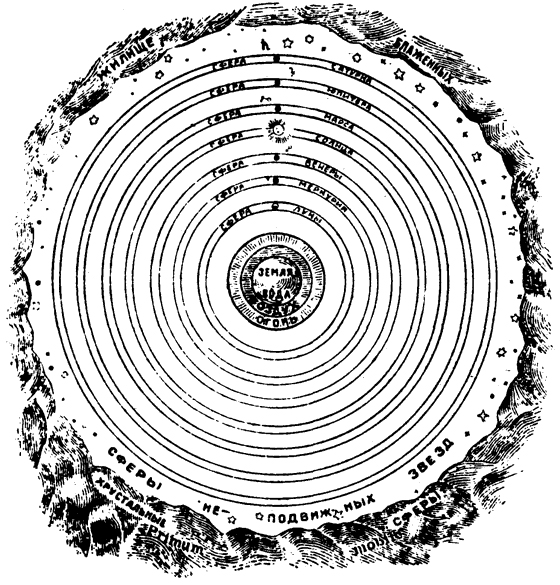
\includegraphics{smp.jpg}}
\end{center}
\caption{Система мира Птолемея.}
\end{figure}
%%\twocolumn

В III веке до н.э. Аристарх Самосский предложил систему, тождественную будущей системе Коперника: Земля и все планеты вращаются по окружностям вокруг неподвижного Солнца. Противниками Аристарха стали Архимед и Аполлоний Пергский, ибо система Аристарза противоречила астрономическим наблюдениям --- во II веке до н.э. это строго доказал Гиппарх. Оба ученых, Аристарх и Гиппарх, были одновременно правы и неправы: Земля и планеты вращаются вокруг Солнца, но не по окружностям, а по эллипсам! Казалось бы, до истины остался один шаг. Но шаг этот не удалось сделать не только Копернику, но и Галилею. Окружности в качестве орбит планет казались абсолютно бесспорными: они были единственными совершенными кривыми. Андрэ Бонар в ``Греческой цивилизации'', вышедшей в 1959 году, пишет: ``Жаль, что ученые, которые возражали Аристарху, не пришли к открытию Кеплера. Но предрассудок о превосходстве кругообразного движения прочно укоренился''.

Слова древних об обязательности совершенства орбит кажутся смешными. Переведем, однако, эти слова на современный язык. Одной из ведущих идей современной физики, как уже было сказано, является идея об однородности и изотропии пространства. Из этой идеи вытекают основные законы физики. Но ведь если орбита планеты не является круговой, то в пространстве появляется выделенное направление наибольшей вытянутости орбиты, которое оказывается чем-то отличным от всех остальных направлений! То, что движение планет обусловлено их предысторией, было еще непостижимо.

\begin{figure}[ht]
\begin{center}
\resizebox{\columnwidth}{!}{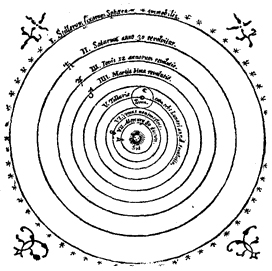
\includegraphics{smk.jpg}}
\end{center}
\caption{Система мира Коперника.}
\end{figure}

Поэтому Птолемей (II вед н.э.) исходит из геоцентрической системы и, вводя сложную картину круговых орбит, объясняет все наблюдаемые факты. Более того, он получает возможность предсказывать движение планет и даже затмения Солнца и Луны. Это так поразило воображение древних, что его сочинение получило имя ``Альмагест'' --- величайшее. Птолемей стал первым в истории астрономом, которому удалось согласовать астрономические наблюдения со своей теорией. Великое достижение! Но, возможно, именно оно на многие века затормозило выяснение истинного движения планет: ведь все так хорошо, теория так прекрасно совпадает с экспериментом!

\begin{figure}[ht]
\begin{center}
\resizebox{\columnwidth}{!}{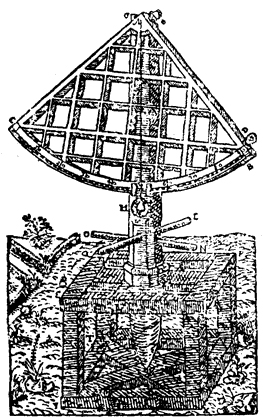
\includegraphics{ktb.jpg}}
\end{center}
\caption{Квадрант Тихо Браге.}
\end{figure}

Проходит 17 веков, и история повторяется! Каноник Фрауэнбургского собора Николай Коперник стремится всего лишь привести систему Птолемея в соответствие с наблюдениями своего времени и замечает: систему Птолемея можно несколько упростить, если считать, что Земля и планеты вращаются вокруг Солнца, но по-прежнему по сложной системе окружностей. И опять, как и у Аристарха, у Коперника есть оппонент --- один из величайших астрономов-наблюдателей всех времен Тихо Браге. Он отвергает систему Коперника примерно по тем же причинам, что и Гиппарх систему Аристарха много веков назад. Тихо Браге не может принять столь усложненную, негармоничную систему мира. Требование гармонии у Браге имеет столь же глубокое значение, как требование совершенных орбит у Архимеда и Гиппарха. Должны существовать основные законы природы, которые не могут не быть простыми. Конечно, это эстетическое утверждение невозможно доказать, но оно вряд ли вызовет улыбку, если вспомнить, что простоту и изящество законов в качестве одного из критериев их истинности предлагал Эйнштейн!

И тут в истории науки появляется Кеплер, преемник Тихо Браге. Начинается новый тур научного поединка. Обработак наблюдения Браге (именно они составили фундамент для построения правильной картины Солнечной системы) и добавив к ним свои собственные наблюдения, Кеплер первым в истории человечества понял устройство Солнечной системы. После долгих безуспешных попыток найти гармонию мира в системе правильных многогранников, заключающих орбиты планет, Кеплер приходит к великому закону: планеты движутся вокруг Солнца, но движутся по эллипсам!

\begin{figure}[ht]
\begin{center}
\resizebox{\columnwidth}{!}{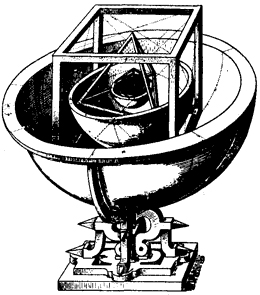
\includegraphics{km.jpg}}
\end{center}
\caption{Модель вселенной Кеплера, предположенная им первоначально.}
\end{figure}

В этом законе проявилась не только готовность Кеплера высказать столь безумную идею, отвергающую взгляды двадцати веков. Кеплеру еще необычайно повезло. Благодаря огромной удаленности планет (особенно тяжелых) друг от друга их орбиты близки к эллипсу --- одной из трех кривых, хорошо известных в то время (эллипс, гипербола, парабола).

Кеплер первым установил законы движения планет. Как он пришел к своему второму закону: в равные промежутки времени планеты описывают равные площади,---остается почти непостижимым. Ведь интегрального исчисления еще не существовало, и вычисление площадей было не столько наукой, сколько искусством: каждая кривая требовала своего подхода. Откуда вообще могла появиться мысль о совершенно необычном законе площадей? Вероятно, сказалось и раннее увлечение Кеплера---изобретенные им в труде ``О стереометрии винных бочек'' (гений из прикладной задачи создает науку!) конкретные методы выичслений площадей, и почти мистическая вера в существование единых законов природы\footnote{Кеплер был глубоко верующим человеком и ушел из богословия в астрономию, утешив себя тем, что ``бога можно прославлять не только богословием''. Но из учебника астрономии, написанного благочестивым Кеплером, бог выпал, и книга была сразу же внесена католической церковью в список запрещенных. Таков частый итог честного служения истине.}, и, вероятно, просто любовь к вычислениям ради вычислений, и то, что называется гениальностью\footnote{Нельзя не назвать хотя бы некоторые работы Кеплера: третий основной закон движения планет, послуживший Ньютону основой для вывода закона всемирного тяготения (!); объяснение приливов и отливов; идея о световом давлении (!), создающем хвосты комет; предсказание спутников Марса и астероидов; установление одного из важнейших положений дифференциального исчисления---условия максимума функции.}.


\begin{figure}[ht]
\begin{center}
\resizebox{\columnwidth}{!}{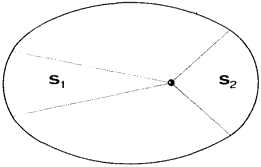
\includegraphics{kl.jpg}}
\end{center}
\caption{Второй закон Кеплера: $S_1=S_2$.}
\end{figure}

Непримиримым научным проивником Кеплера стал его современник Галилей. Он первый поставил вопрос о том, что же движет планеты, заставляя их орбиты искривляться. Воздействие Солнца на таком расстоянии Галилей считал мистикой, как и связь приливов с Луной. Откуда планеты знают, что в следующий час они должны описать такую же площадь, как и в предыдущий?\footnote{Поучительно сравнить этот вопрос с вопросом Резерфорда Бору: откуда электрон знает, какой частоты свет он должен излучать, перескакивая на новую орбиту?} Требовалась принципиально новая постановка вопроса, потому что неправилен был сам привычный вопрос. А ответ Кеплера: ``Планеты движет мировая душа'', разумеется, не мог удовлетворить Галилея. Но раз силы, действующей на планеты, не существует, рассуждал Галилей, значит, подобное движение---естественное свойство планет. Галилей назвал его инерцией и очень убедительно доказал ошибочное утверждение: причина вращения планет---инерция, движение по инерции может быть только движением по окружности, все точки которой равноправны(!).

Движение по прямой Галилей полагал исключенным: переход со временем из одной точки в другую означал бы их неэквивалентность; кроме того, в этом случае тело никогда не достигло бы конечной цели (на современном языке---равновесного устойчивого состояний), а природа никогда не ставит себе недостижимых целей (то есть равновесное состояние рано или поздно наступает).

Это рассуждение привело Галилея к противоречию не только с Кеплером, но и с самим собой: ведь ранее он доказал, что движение по кругу связано с силой, действующей к центру! Противоречие казалось неразрешимым, а Декарт сделал ситуацию еще более драматичной, показав, что движение по инерции---это движение по прямой.

Что же движет планеты?

Выхода, казалось, не было. Но в год смерти Галилея родился Ньютон. Он вернулся к Кеплеру, к его законам, и на их основе создал точную науку о движении тел.

До сих пор речь шла только о столкновении идей, о спорах между рыцарями мысли: Филолаем и Аристотелем, Аристархом Самосским и Гиппархом, Коперником и Тихо Браге, Кеплером и Галилеем, спорах, в которых выяснилось, что истина еще не родилась. Но ведь ученые---живые люди, с их страстями, самолюбием, гордостью и способностью ошибаться даже в малом. Галилей был убежден в невозможности покинуть Землю и не заметил, что его формулы давали первую космическую скорость\footnote{Кстати, а \uline{как, используя формулу} $S=gt^2 / 2$,\uline{получить выражение для первой космической скорости?}}. Он объяснял приливы движением Земли вокруг Солнца (так хотелось первому указать явление, доказывающее это движение!), но период приливов вдвое отличался от его расчетов и совпадал с результатами Кеплера. Галилей объявил совпадение у Кеплера случайностью\footnote{Вспомним Бора: ``Совпадение дурацкой теории с экспериментом еще ничего не доказывает, существует бесчисленное множество таких теорий''.}, а сам наивно и беспомощно апеллировал к слухам, что где-то в Саргассовом море период приливов ``правильный''. Но одновременно он пытается связать неправильный период прилива в Средиземном море с его глубиной---и создает новую область науки: изучение поверхностных волн и волн в замкнутых бассейнах! Галилей открыл независимость периода колебаний маятника от амплитуды---и тут же, увлекшись, ошибочно распространил этот закон на любую величину амплитуды; обнаружил постоянство земного ускорения---и немедленно сделал вывод о его независимости от расстояния до Земли! Так ошибался основатель чуть ли не всех областей механики\footnote{О суетности гениев. Ньютон из научной добросовестности 20 лет не публиковал свой закон всемирного тяготения, стремясь вывести из него законы Кеплера, а потом долгие годы спорил о приоритете с Гуком; не публиковал свое открытие дифференциального и интегрального исчислений, пытаясь найти общую формулу для интеграла, а затем доказывал свой приоритет в споре с Лейбницем. Ибо Ньютон жил только наукой, всю жизнь был одинок и не мог пожертвовать своей единственной житейской радостью---славой, хотя славы его открытий хватило бы на многих.}.

Так, в густой смеси прозрений и заблуждений, без правых и неправых развивалась наука. А ведь при этом все, о ком шла речь, были гениями: их труды служат уже несколько веков; они продвинули все человечество на много десятилетий вперед (а чем, как не числом сэкономленных человеко-лет, определяется степень таланта?); большое время ушло на понимание и освоение их идей---великая истина редко рождается простой и понятной\footnote{Вот, например, правило умножения из рукописи XV века: $7\times8=?$ $7+8-10=5$, далее $5\times10=50$, теперь определим $10-7=3$, $10-8=2$ и перемножим эти результаты: $3\times2=6$. Наконец, $50+6=56$, так что $7\times8=56$.}.

Изложенная история развития науки, конечно, крайне упрощена и написана грубыми мазками, иногда с нарочитой конденсацией фактов. Но ясно, что развитие идет не по прямой телеграфного столба, а скорее по сложной кривой дерева науки, ветви которого наклонены под разными углами к истине и постепенно спрямляются, чтобы подняться на новый ярус знания.

\section*{Ответы, указания, решения}

\emph{К статье ``Закон инерции, гелиоцентрическая система и развитие науки''}
\begin{small}
\begin{enumerate}
\item Если бы исчезло притяжение Солнца, центр тяжести Земли стал бы двигаться по касательной к орбите. Вращение Земли вокруг оси сохранилось бы.
\item Шарик начинает кататься по полу трамвая, когда появляется ускорение.
\item Тело брошенное горизонтально со скоростью $v$ с высоты $h$ наз Землей, за малое время $t$ пройдет по направлению скорости расстояние $x=v*t$ и в перпендикуляром направлении расстояние $\Delta h=gt^2/2$, оказавшись на некоторой высоте $h_1$ над Землей. Если $h=h_1$, то тело вращается вокруг Земли по круговой орбите. Вычислив $h_1$ и полагая $h=h_1$, найдем, что $v$ должна быть равна $\sqrt{gR}$
\end{enumerate}
\end{small}

%%\section*{Кому что понятно}
%%Выдающийся русский геометр и педагог А.~К.~Власов, изложив на очередной лекции по аналитической геометрии задачу о пересечении двух прямых, заданных своими уравнениями, добавил:
%%
%%---Два студента, впервые ознакомившиеся с этим вопросом, беседовали между собою.
%%
%%Один сказал: ``Теперь я понял, почему система двух уравнений первой степени с двумя неизвестными имеет в общем случае одно решение. Это потому, что две прямые пересекаются в одной точке''.
%%
%%Другой ответил: ``Вот когда я, наконец, понял, почему две прямые пересекаются в одной точке! Это потому, что система двух уравнений первой степени с двумя неизвестными имеет одно решение''.

\end{document}
